% Document Type
\documentclass[a4paper,11pt]{article}

% Packages
\usepackage{latexsym}
\usepackage[empty]{fullpage}
\usepackage{titlesec}
\usepackage{marvosym}
\usepackage[usenames,dvipsnames]{color}
\usepackage{verbatim}
\usepackage{enumitem}
\usepackage{fancyhdr}
\usepackage[english]{babel}
\usepackage{tabularx}
\usepackage{graphicx}
\usepackage{color}
\usepackage[table]{xcolor}
% \usepackage{tgbonum}
\usepackage[sfdefault]{ClearSans} %% option 'sfdefault' activates Clear Sans as the default text font
\usepackage[T1]{fontenc}
\usepackage[margin=1.4in]{geometry}
\usepackage{setspace}
\usepackage{multirow}
\usepackage[hidelinks]{hyperref}
\input{glyphtounicode}

% Cover Information
\title{Ling Li Ya CV}
\author{Ling Li Ya}
\date{\today}


\pagestyle{fancy}
\fancyhf{} % clear all header and footer fields
\fancyfoot{}
\renewcommand{\headrulewidth}{0pt}
\renewcommand{\footrulewidth}{0pt}


% My Colours
\definecolor{MyBlue}{rgb}{0.17, 0.27, 0.59}
\definecolor{MyBGColor}{rgb}{0.90, 0.94, 0.98}
\definecolor{MyHighlight}{rgb}{1.00, 0.89, 0.00}


% URL
\hypersetup{breaklinks=false,%
% pagecolor=white,%
colorlinks=true,%
linkcolor=MyBlue,%
anchorcolor=MyBlue,%
urlcolor=MyBlue}
\urlstyle{same}


% Adjust margins
\addtolength{\oddsidemargin}{-0.5in}
\addtolength{\evensidemargin}{-0.5in}
\addtolength{\textwidth}{1in}
\addtolength{\topmargin}{-0.7in}
\addtolength{\textheight}{1.0in}

\raggedbottom
\raggedright
\setlength{\tabcolsep}{0in}


% Sections formatting
\titleformat{\section}{
  \vspace{5pt}\raggedright\large\bfseries
}{}{0em}{}[\color{black}\titlerule \vspace{-5pt}]


% Ensure that generate pdf is machine readable/ATS parsable
\pdfgentounicode=1


%-------------------------
% Custom commands
\newcommand{\resumeItem}[2]{
  \item\small{
    \textbf{{#1:} }{#2 \vspace{-2pt}}
  }
}


% Just in case someone needs a heading that does not need to be in a list
\newcommand{\resumeHeading}[4]{
    \begin{tabular*}{0.99\textwidth}[t]{l@{\extracolsep{\fill}}r}
      \textbf{#1} & {#2} \\
      \textit{\small#3} & \textit{\footnotesize #4} \\
    \end{tabular*}\vspace{-5pt}
}


\newcommand{\resumeSubheading}[4]{
  \vspace{-1pt}\item
    \begin{tabular*}{0.97\textwidth}[t]{l@{\extracolsep{\fill}}r}
      \textbf{\color{MyBlue} #1} & {\footnotesize#2} \\
      \textit{\footnotesize #3} & \textit{\footnotesize #4} \\
    \end{tabular*}\vspace{-5pt}
}


\newcommand{\resumeSubSubheading}[2]{
    \begin{tabular*}{0.97\textwidth}{l@{\extracolsep{\fill}}r}
      \textit{\footnotesize #1} & \textit{\footnotesize #2} \\
    \end{tabular*}\vspace{-5pt}
}


\newcommand{\resumeSubItem}[2]{\resumeItem{#1}{#2}\vspace{-4pt}}


\renewcommand{\labelitemii}{$\circ$}


\newcommand{\resumeSubHeadingListStart}{\begin{itemize}[leftmargin=*]}
\newcommand{\resumeSubHeadingListEnd}{\end{itemize}}
\newcommand{\resumeItemListStart}{\begin{itemize}}
\newcommand{\resumeItemListEnd}{\end{itemize}\vspace{-5pt}}


% Own symbols
\newcommand{\CC}{C\nolinebreak\hspace{-.05em}\raisebox{.4ex}{\tiny\bf +}\nolinebreak\hspace{-.10em}\raisebox{.4ex}{\tiny\bf +}}
\def\CC{{C\nolinebreak[4]\hspace{-.05em}\raisebox{.4ex}{\tiny\bf ++}}}
\newcommand{\mytextsharp}{$^\sharp$}


%-------------------------------------------
%%%%%%  CV STARTS HERE  %%%%%%%%%%%%%%%%%%%%%%%%%%%%

\begin{document}

%----------HEADING-----------------
\begin{tabular*}{\textwidth\footnotesize}{ll @{\extracolsep{\fill}}r}
  \multirow{5}{*}{
    \begin{minipage}[l][2.0cm][c]{2.25cm}
      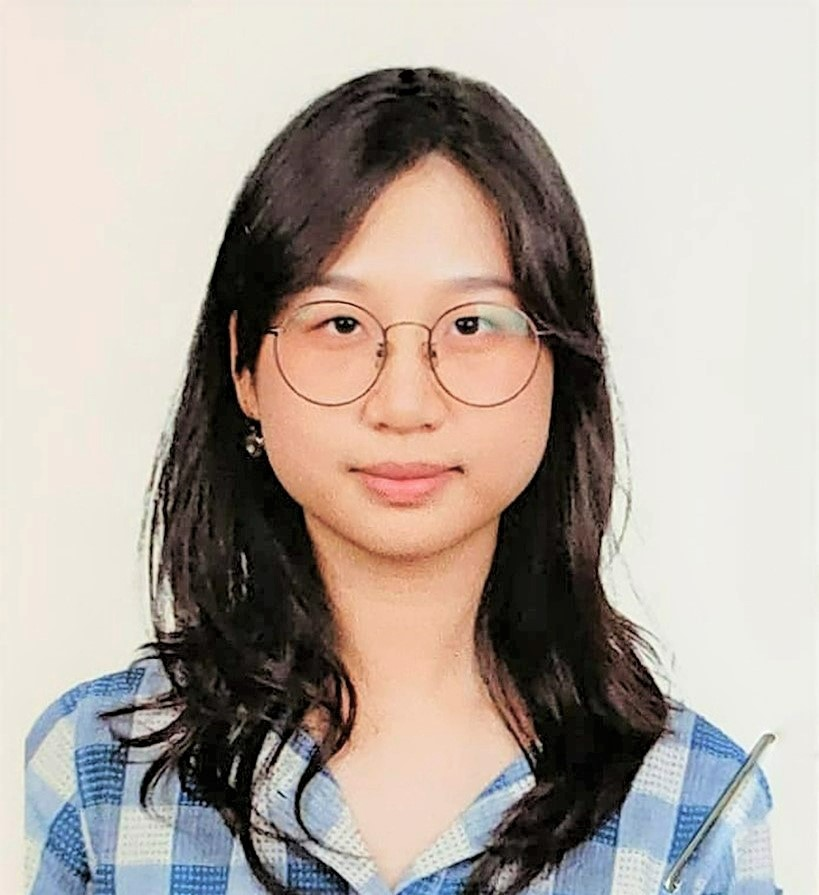
\includegraphics[width=2.0cm]{../profile-pic.jpg}
    \end{minipage}}  & {\textbf{\Large LIANA LING LI YA}} & \\
  & {\textit{Junior Quant Researcher}} & {Email: \textbf{\href{mailto:lianalingliya@gmail.com}{lianalingliya@gmail.com}}} \\
  & {Apr 10, Phoenix Park Racecourse}, & {Mobile: \textbf{\href{tel:+60172801215}{+353 87 248 1446}}} \\
  & {Castleknock, D15 X381, Dublin 15} & {GitHub: \textbf{\href{http://github.com/lianaling/}{github.com/lianaling}}}\\
  & {Dublin, Ireland.} & {This Document: \textbf{\href{https://github.com/lianaling/resume/}{Coded with \LaTeX}}} \\
\end{tabular*}


%-----------Education-----------------
\section{EDUCATION}
\resumeSubHeadingListStart
\resumeSubheading
{University College Dublin}{Dublin, Ireland}
{Masters of Science in Computer Science}{Sep 2023 -- Sep 2024}
% \begin{spacing}{0.4}
%   \colorbox{yellow}{\it\footnotesize CGPA: 3.9744}
% \end{spacing}
\resumeItemListStart
\resumeItem{Skills Acquiring}{Machine Learning, Advanced Machine Learning, Connectionist Computing, Text Analytics, Data Science, Monte Carlo Simulation}
\resumeItem{Languages}{Native-level in written/spoken English and Chinese; Conversational in Malay}
\resumeItemListEnd
\resumeSubheading
{Tunku Abdul Rahman University of Management and Technology}{Kuala Lumpur, Malaysia}
{Bachelor of Computer Science (Honours) in Software Engineering; \colorbox{MyHighlight}{CGPA:3.98/4.00}}{Oct 2019 -- Oct 2022}
% \begin{spacing}{0.4}
%   \colorbox{yellow}{\it\footnotesize CGPA: 3.9744}
% \end{spacing}
\resumeSubSubheading{Foundation in Science; CGPA: 4.00}{Sep 2018 -- Sep 2019}
\resumeItemListStart
\resumeItem{Skills Acquired}{\CC, C\mytextsharp, Java, Python, ASP.NET, SQL, HTML/CSS/Javascript, VueJS, Quasar}
\resumeItemListEnd
\resumeSubHeadingListEnd

%-----------Experience-----------------
\section{EXPERIENCE}
\resumeSubHeadingListStart

\resumeSubheading
{Balaena Quant Sdn Bhd}{Kelana Jaya, Malaysia}
{Junior Quant Researcher}{Dec 2022 -- Sep 2023}
\resumeItemListStart
\resumeItem{Statistical Arbitrage}
{Researched and designed minute-level stats arb algorithms in crypto future derivatives}
\resumeItem{Research and Exploration}
{Assisted in researching options volatility surface and order book imbalance}
\resumeItem{Data Pipeline}
{Written a script to automate large-scale historical data insertion for crypto trading pairs}
\resumeItemListEnd

\resumeSubheading
{Datasonic Smart Solutions Sdn Bhd}{Putrajaya, Malaysia}
{Machine Learning Intern}{June 2022 -- Nov 2022}
\resumeItemListStart
\resumeItem{Academic Research}
{Read through journal papers on speech recognition and computer vision}
\resumeItem{Data Preparation}
{Categorised, labelled and augmented 4000 image data using CVAT}
\resumeItem{Model Training}
{Trained YOLOv7 to perform card and landmark detection with mAP@.5 of 0.998 using PyTorch}
\resumeItem{UI/UX Design}
{Designed UI for an OAuth system while connecting to backend services using VueJS and Quasar}
\resumeItemListEnd

\resumeSubheading
{LS SMART MACHINERY (M) SDN BHD}{Seri Kembangan, Malaysia}
{Junior Software Developer}{May 2021 -- Jun 2021}
\resumeItemListStart
\resumeItem{Requirement Elicitation}
{Communicated and documented stakeholder requirements}
\resumeItem{Project Reporting}{Researched and reported on competitor analysis and project costing}
\resumeItem{Database Design}
{Designed, documented and implemented PostgreSQL database schema}
\resumeItem{Backend Setup}{Connected application to Stripe API using Golang and Fiber.ctx}
\resumeItemListEnd

\resumeSubheading
{RSBAITAI by Turcomp BMB SDN BHD}{Work from home, Malaysia}
{Chinese-English Translator-cum-Proofreader}{May 2020 -- Nov 2021}

\resumeSubheading
{Chill Solutions}{Work from home, Malaysia}
{Senior Translator-cum-Proofreader}{Nov 2019 -- May 2020}
\resumeSubSubheading{Junior Translator-cum-Proofreader}{Aug 2019 -- Oct 2019}
\resumeSubHeadingListEnd


%-----------Projects-----------------
\section{PROJECTS}
\resumeSubHeadingListStart
\resumeSubheading{\href{https://github.com/marcustut/fyp}{SliGen, AI Automatic Slide Generator}}{Natural Language Processing}
{Transformer, Python, Flask}{Oct 2021 -- Mar 2022}
\resumeItemListStart
\resumeItem{Model Training}{Fine-tuned a HuggingFace T5 model on the ArXiV dataset for title generation}
\resumeItem{Core Algorithm Implementation}{Summarised text using transformers, converted into Markdown and generated slides via SliDev API}
\resumeItem{API Construction}{Constructed API interface with Flask for linking to web-based application}
\resumeItemListEnd

\resumeSubheading{\href{https://github.com/lianaling/cataclysm}{Cataclysm, Cat Detector}}{Image Processing}
{Haar Cascade Classifier, Python, Threading}{7th Mar 2022}
\resumeItemListStart
\resumeItem{Cat Frontal Face Detection}{Processed frames from IP camera via Android phone with haar cascade classifier}
\resumeItem{Threading}{Started two threads to delay notifications sent via Telegram Bot API}
\resumeItemListEnd

\resumeSubheading{\href{https://github.com/marcustut/summarize}{Summarize, AI Text Summariser}}{Natural Language Processing}
{Transformer, Python, Jupyter Notebook}{Sep 2021 -- Oct 2021}
\resumeItemListStart
\resumeItem{Research and Implementation}{Read through 20+ journal papers and applied 3 abstractive summarisation algorithms}
\resumeItem{Experiment Design}{Designed an experiment, curated relevant dataset, tested algorithms and produced a comparison report that eventually received 98/100 marks}
\resumeItemListEnd
\resumeSubHeadingListEnd


%-----------Academia-----------------
\section{ACADEMIA}
 {\small
  \begin{itemize}[leftmargin=*]{\footnotesize}
    \item{Ling, L., Amirul Imran Ahmad Azam, Ramanathan Palaniappan, \& Tin, T.T. (2021, November 25-27) \textit{Artificial Intelligence Art: Attitudes and Perceptions Toward Human Versus Artificial Intelligence Artworks.} [Paper presentation]. ICHESMET 2021. \vspace{-2pt}}
  \end{itemize}
 }


%-----------Achievements-----------------
\section{ACHIEVEMENTS}
\resumeSubHeadingListStart
\resumeSubItem{TAR UMT President's Award}{Top student with best academic and co-curricular performance}
\resumeSubItem{International English Language Testing System (IELTS) 2022}{Band 8.5 on a 9-band scale}
\resumeSubItem{TAR UMT President's List certificates}{For GPA 3.9000 and above}
\resumeSubItem{TAR UMT Certificate in Soft Skills}{For foundation and bachelor's degree}
\resumeSubItem{Secondary School Awards}{Most Disciplined Student, Highest Average Score, Highest Number of Modules Completed in 2015, 2016 and 2017}
\resumeSubHeadingListEnd


%-----------Activities-----------------
\section{ACTIVITIES}

\resumeSubHeadingListStart
\resumeSubheading{Taman Sri Muda Flood Relief}{TAR UMT/Shah Alam Gospel Centre}{Volunteer}{24th, 27th Dec 2021}
\resumeSubheading{Google \#GCPBoleh}{Google}{Self-Learning Student}{Oct 2021 -- Nov 2021}
\resumeItemListStart
\resumeItem{Tutorial}{Completed 5 Machine Learning and 1 BigQuery Data tutorials on GCP}
\resumeItemListEnd
\resumeSubheading{Google Developer Student Club TAR UMT}{Google}
{Marketing \& Creative Lead}{Jan 2021 -- Oct 2021}
\resumeItemListStart
\resumeItem{Account Management}{Managed communication channels on 5 social media accounts}
\resumeItem{Poster and Caption Design}{Created event posters and relevant captions}
\resumeItem{Event Hosting}{Hosted and facilitated the event \textit{Meet the Xperts: A Journey in the IT Industry}}
\resumeItemListEnd
\resumeSubHeadingListEnd


%-------------------------------------------
\end{document}

% -----Credits-----
% Template: Sourabh Bajaj
% License : MIT